\documentclass[12pt,a4paper]{article}
\usepackage{physics}
\usepackage{amssymb}
\usepackage{subcaption}
\usepackage{colortbl}
\input{spp.dat}
\fancyhead[c]{Activity 5 -- Enhancement by Histogram Manipulation}

%  Editorial staff will uncomment the next line
% \providecommand{\artnum}[0]{XX-XX}
% \renewcommand{\articlenum}[0]{SPP-\the\year-\artnum-}

\begin{document}

\title{\TitleFont Activity 5 -- Enhancement by Histogram Manipulation}
\author[ ]{\textbf{Kenneth V. Domingo} \\
2015--03116 \\
App Physics 186, 1\textsuperscript{st} Semester, A.Y. 2019--20}
\affil[ ]{\corremail{kvdomingo@up.edu.ph} }

\maketitle
\thispagestyle{titlestyle}

\section*{Results and Discussion}
\setcounter{section}{1}

For this activity, I chose a low-light portrait that I shot at the Light Bridge at the Mind Museum (Fig. \ref{fig:orig}) last April. I imported it as \texttt{uint8} for ease in the histogram manipulation later on (something to do with indexing). Its histogram is shown in Fig. \ref{fig:orig-hist}. Notice that the histogram values range only from 0 to 226. The ``spike'' at the end most likely corresponds to the clipped highlights evident in the light stripes that can be seen in the original, unprocessed image. This spike is also reflected in its CDF, shown in Fig. \ref{fig:orig-cdf}.

The first order of business is contrast stretching, which is essentially stretching the histogram so that it encompasses the entire data space available for the data type, in this case, 0 to 255. We first convert the image to \texttt{float32} by dividing it by 255 in order to constrain the pixel values between 0 and 1. Since the global maximum of the original image is 226, no pixel will have an exact value of 1. We want to stretch the data so that its maximum is exactly 1, so we transform the pixel intensities according to \cite{soriano}:

\begin{equation}\label{eq:constrast-stretch}
	I'(x,y) = \frac{I(x,y) - I_{\min}}{I_{\max} - I_{\min}}
\end{equation}

We then cast the image back into \texttt{uint8} by multiplying by 255 and rounding off. The result of this process is shown in Fig. \ref{fig:cs}. At face value, there is no discernible change since the global maximum of the original image is fairly close to 255. However, in the eyes of a photographer, there are substantial contrast \& detail enhancements, particularly in the regions with rapid light falloff, such as on the shirt. If you zoom in quite a bit, the side of the face which is better lit has more pronounced details. The light stripes also appear less clipped, and are now a tad brighter. Looking into its histogram (Fig. \ref{fig:cs-hist}), we see that the brighter range of pixels are now more even, and now encompass the full range of values up to 255, and the ``stretching'' is evident by the lack of some pixels in the lower range. The CDF (Fig. \ref{fig:cs-cdf}) also reflects a smoother increase in the upper range of values.

Next, we perform histogram equalization. Generating the desired CDF (Fig. \ref{fig:histeq-cdf}) is trivial: we just use $G(z) = z$ in the range $[0, 255]$ for both $x$ and $y$ axes since we intend to retain its data type. By importing the image as an unsigned integer type, it makes the job of backprojection much easier as we only need to take the pixel values of the original image and use that as an index to find the corresponding pixel value in the desired CDF. The resulting image is shown in Fig. \ref{fig:hist-eq}. We can see from its histogram in Fig. \ref{fig:histeq-hist} that the pixel values are now uniformly spread out throughout the data range. Since the bulk of the pixel values were originally in the lower range, the image now looks more properly exposed, albeit less in contrast.

Finally, we try to simulate a nonlinear response by generating a sigmoid CDF (Fig. \ref{fig:adapteq-cdf}) of the form

\begin{equation}\label{eq:sigmoid}
	G(z) = \frac{1}{1 + e^{-z}}
\end{equation}

\noindent
and scaling it to \texttt{uint8} then rounding off. The resultant image can be seen in Fig. \ref{fig:adapt-eq}, and its histogram in Fig. \ref{fig:adapteq-hist}. Once again, the image appears more properly exposed, but now is high in contrast. We can also see in the histogram that the middle values are stretched more than the outer values.

Upon further reading, this is actually the method used for a technique called adaptive equalization \cite{skimage}. The CDF is a nonlinear response, usually of a sigmoid-like shape which is shifted along the $x$ axis and/or varied in slope, depending on where most of the original pixel values are clustered, and I generally use this to correct the exposure of images without blowing out the highlights or crushing the shadows. I also recognized the $S$-curve of the CDF and its effect on the image, and I realized that the CDF is actually what is called the tone curve in photo editing programs such as Lightroom and Photoshop. To test this, I tried to perform a technique called ``crushing the blacks/whites'', which is used to simulate a faded film look, wherein the tone curve is shaped like a sigmoid, but the endpoints are clipped, i.e., the global minimum should be $> 0$ and the global maximum should be $< 255$, sort of like the opposite of contrast stretching. To do this, I generated a sigmoid CDF (Fig. \ref{fig:crush-cdf}) with a bias and scaled it to a value less than 255, so that its minimum and maximum $y$ values are 42 and 197, respectively. Using the same process as before, lo-and-behold, I got the expected result in Fig. \ref{fig:crushed}, and it definitely looks like it was taken with the classic Kodak Tri-X film. Its histogram in Fig. \ref{fig:crush-hist} also shows the squeezing of the pixel values and confirms that the technique acts like \textit{contrast compressing}.

\begin{figure}[htb]
    \centering
	\begin{subfigure}[h!]{0.24\textwidth}
		\centering
		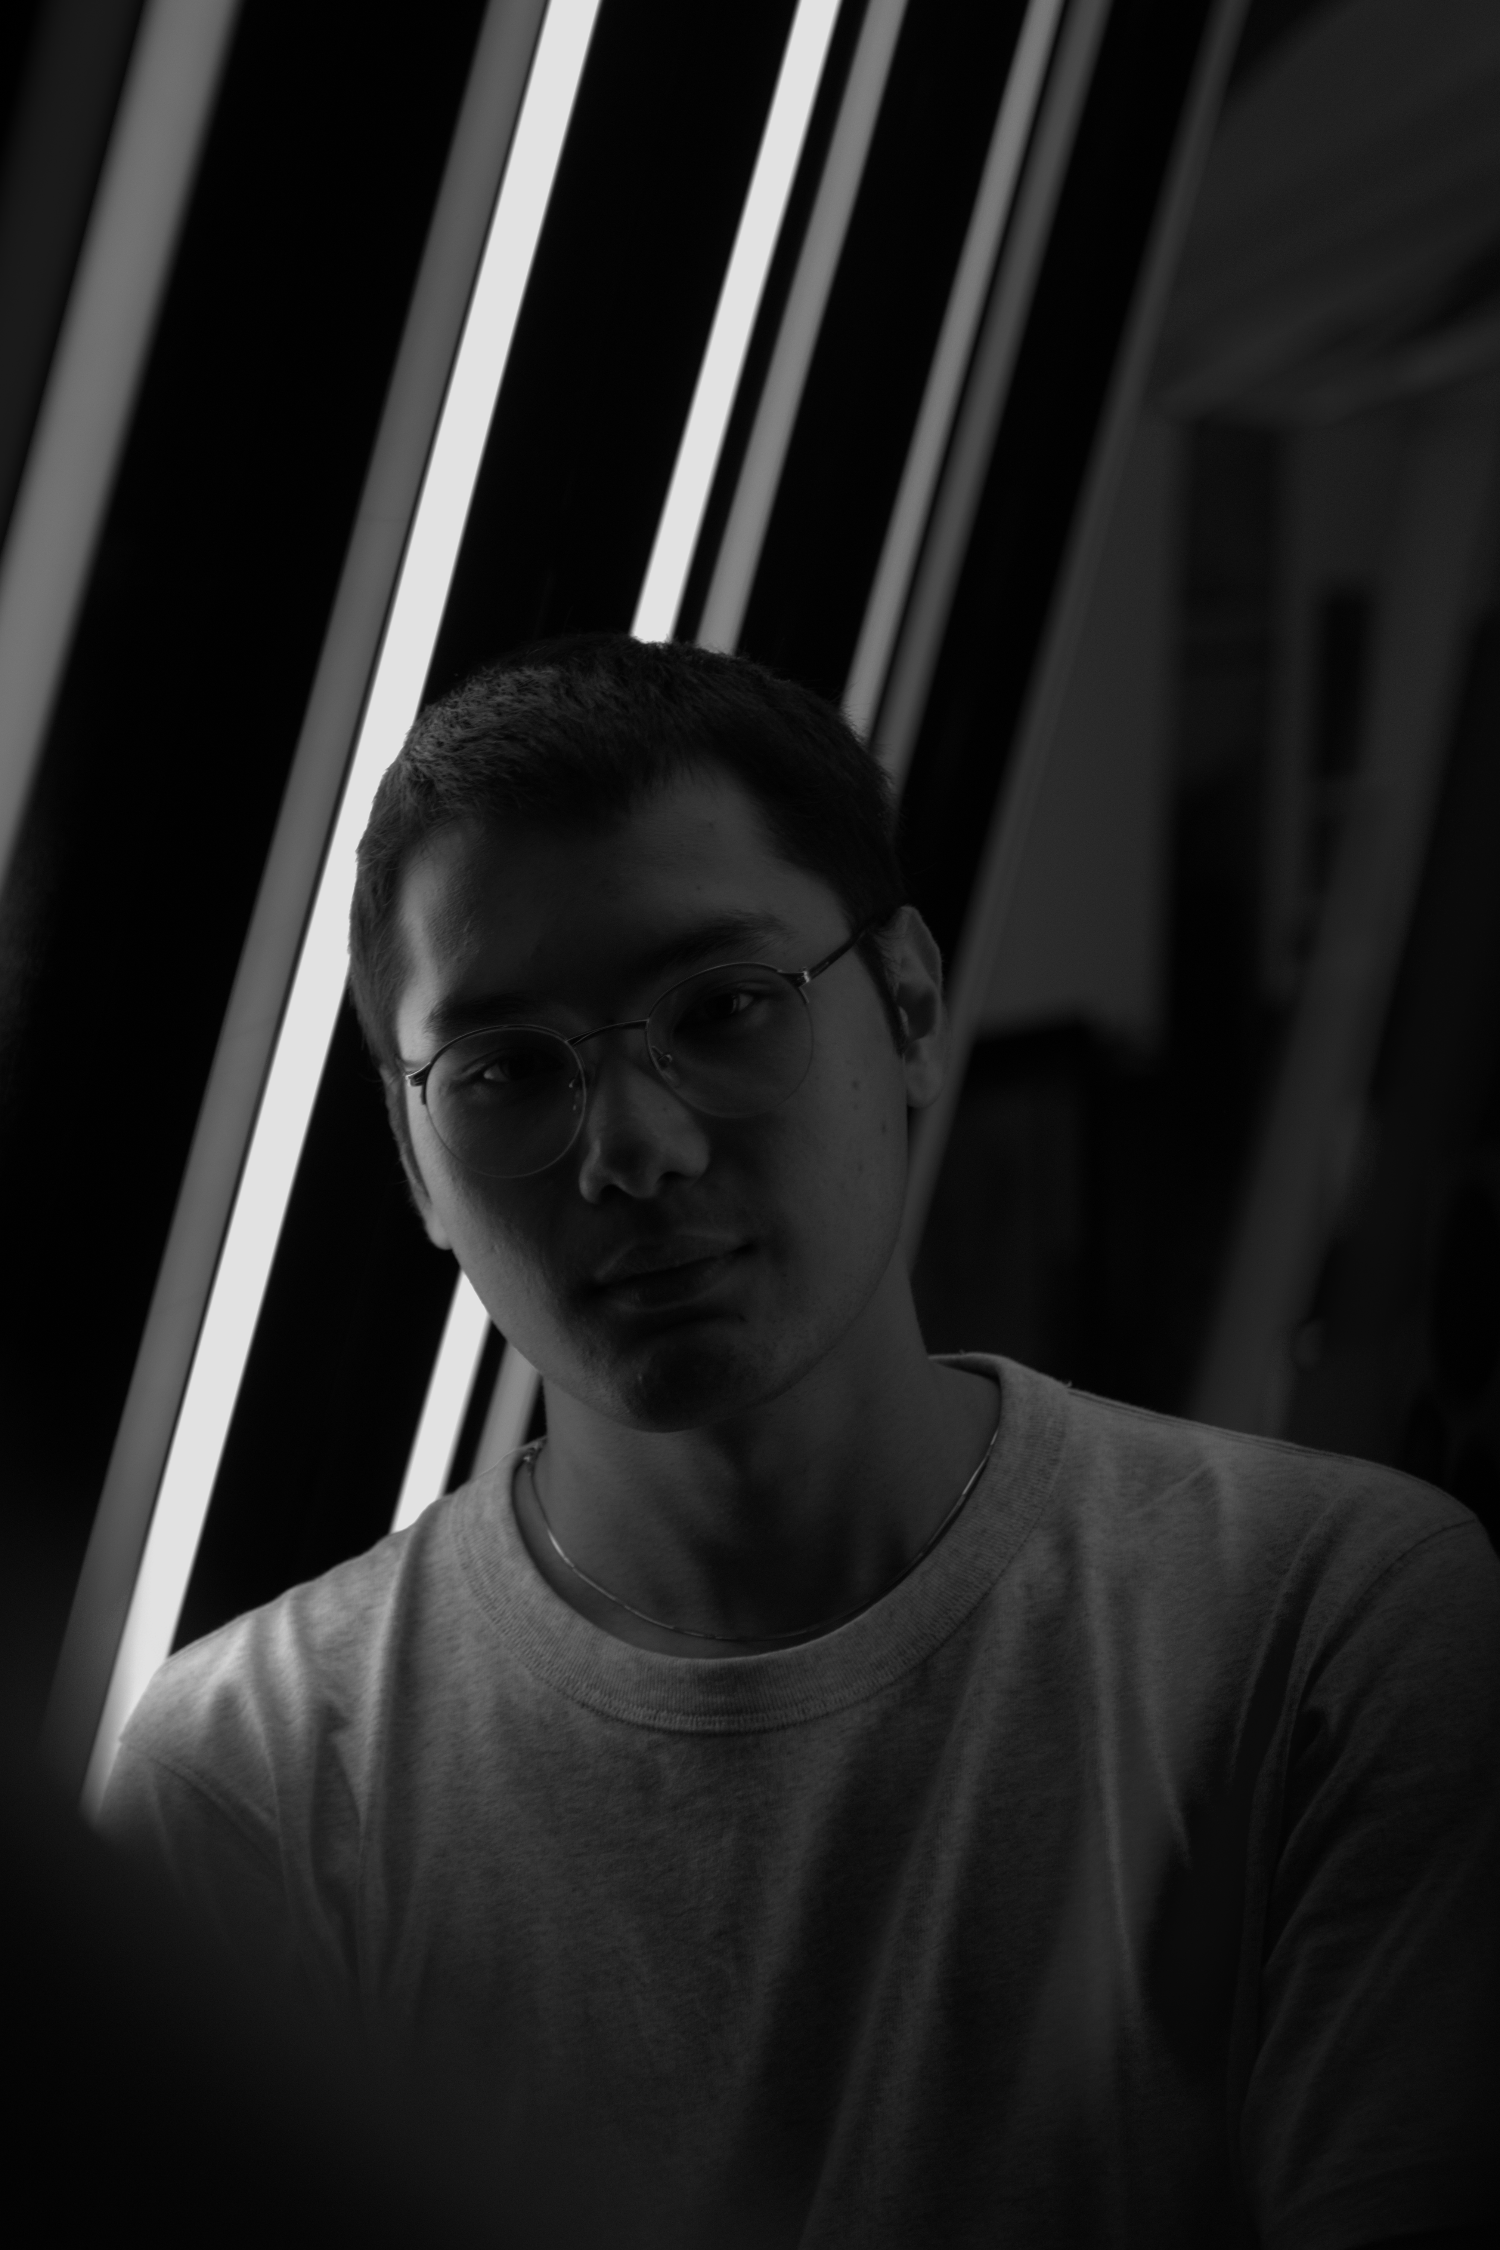
\includegraphics[width=\textwidth]{original.png}
		\caption{Original}
		\label{fig:orig}
	\end{subfigure}
	\begin{subfigure}[h!]{0.24\textwidth}
		\centering
		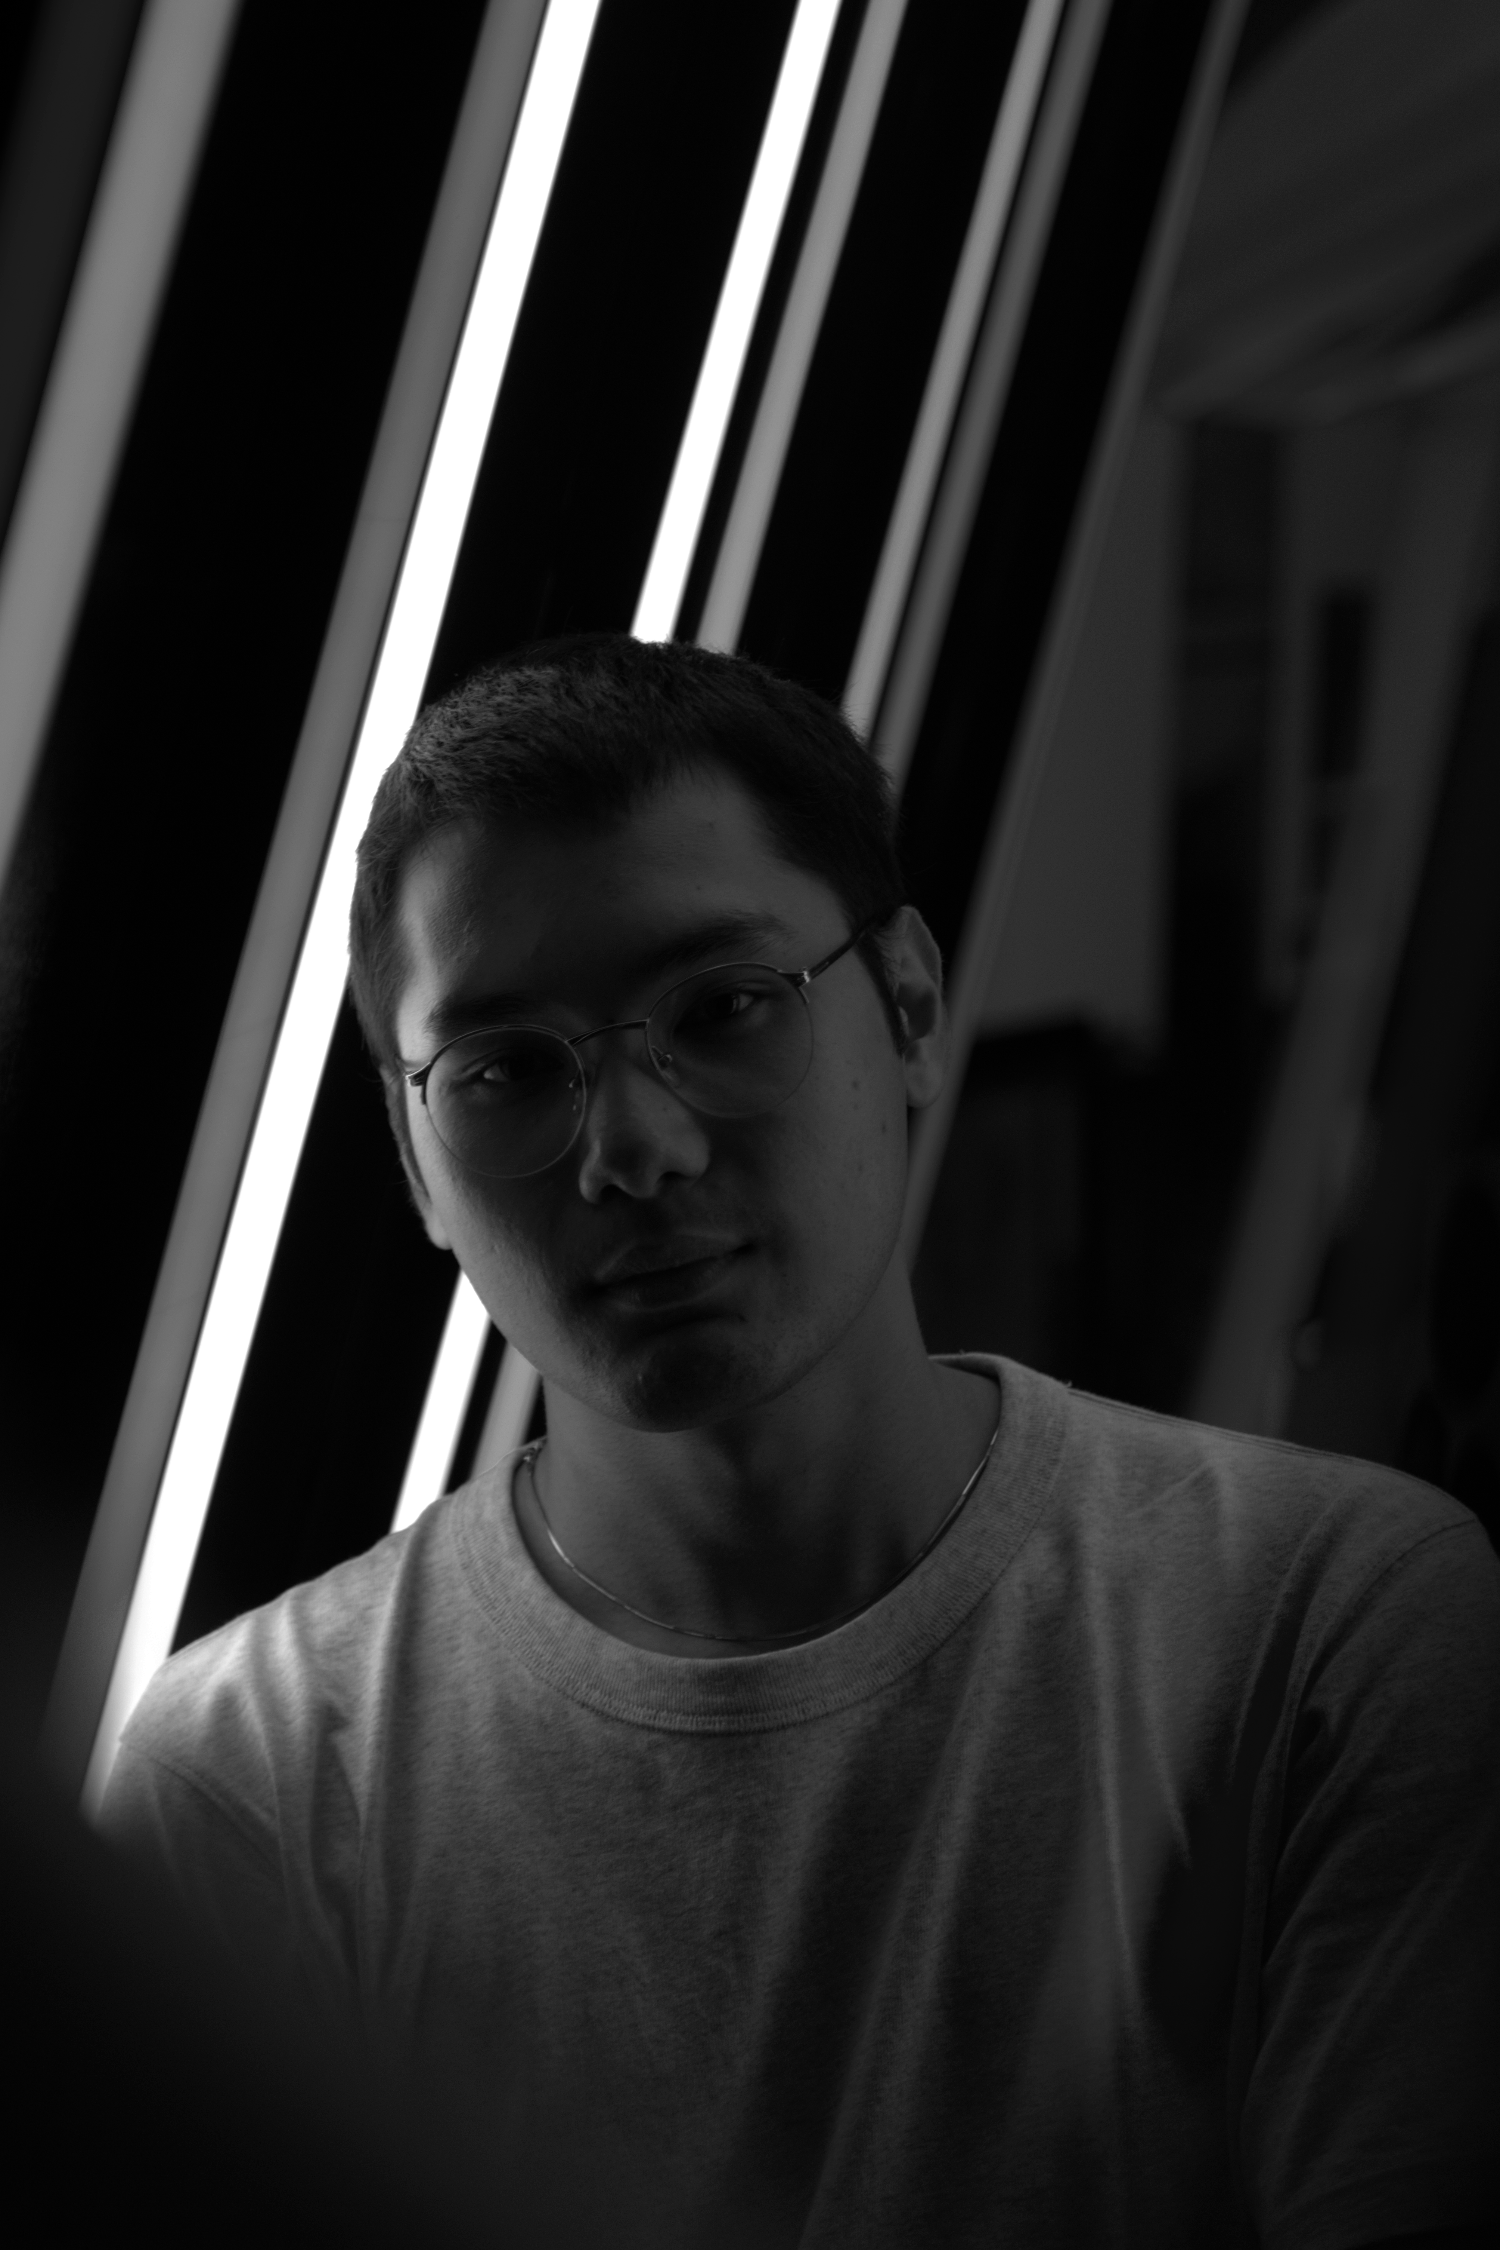
\includegraphics[width=\textwidth]{contrast_stretch.png}
		\caption{Contrast-stretched}
		\label{fig:cs}
	\end{subfigure}
	\begin{subfigure}[h!]{0.24\textwidth}
		\centering
		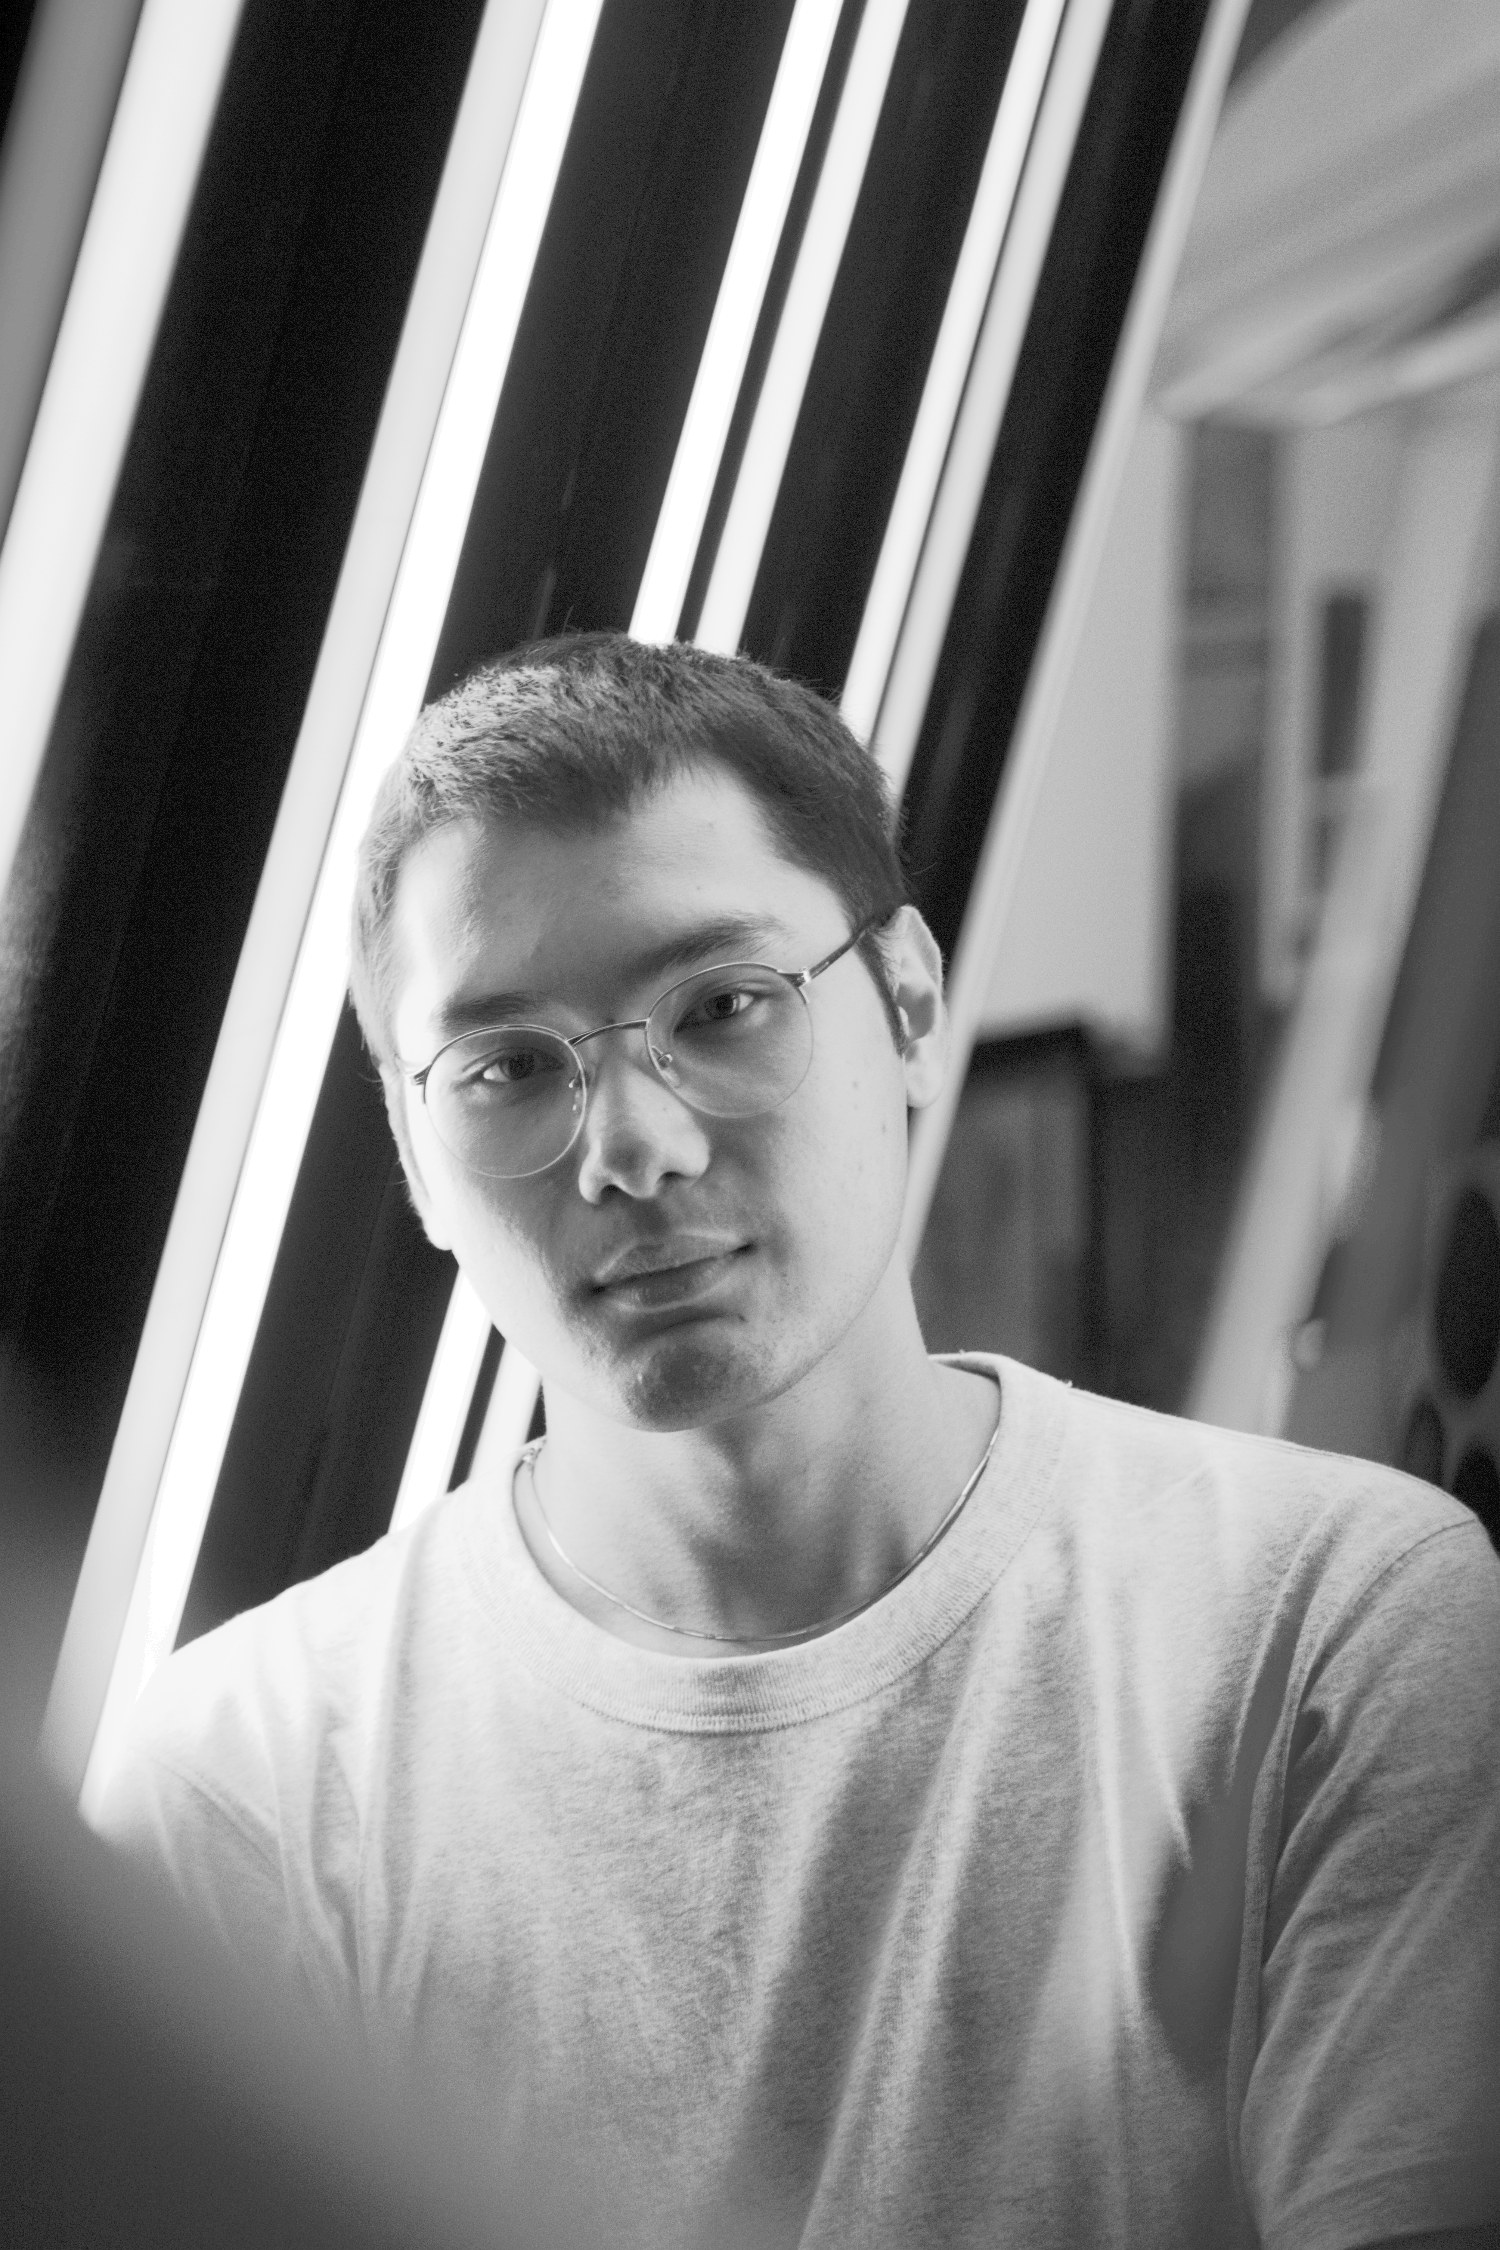
\includegraphics[width=\textwidth]{hist_equal.png}
		\caption{Histogram-equalized}
		\label{fig:hist-eq}
	\end{subfigure}
	\begin{subfigure}[h!]{0.24\textwidth}
		\centering
		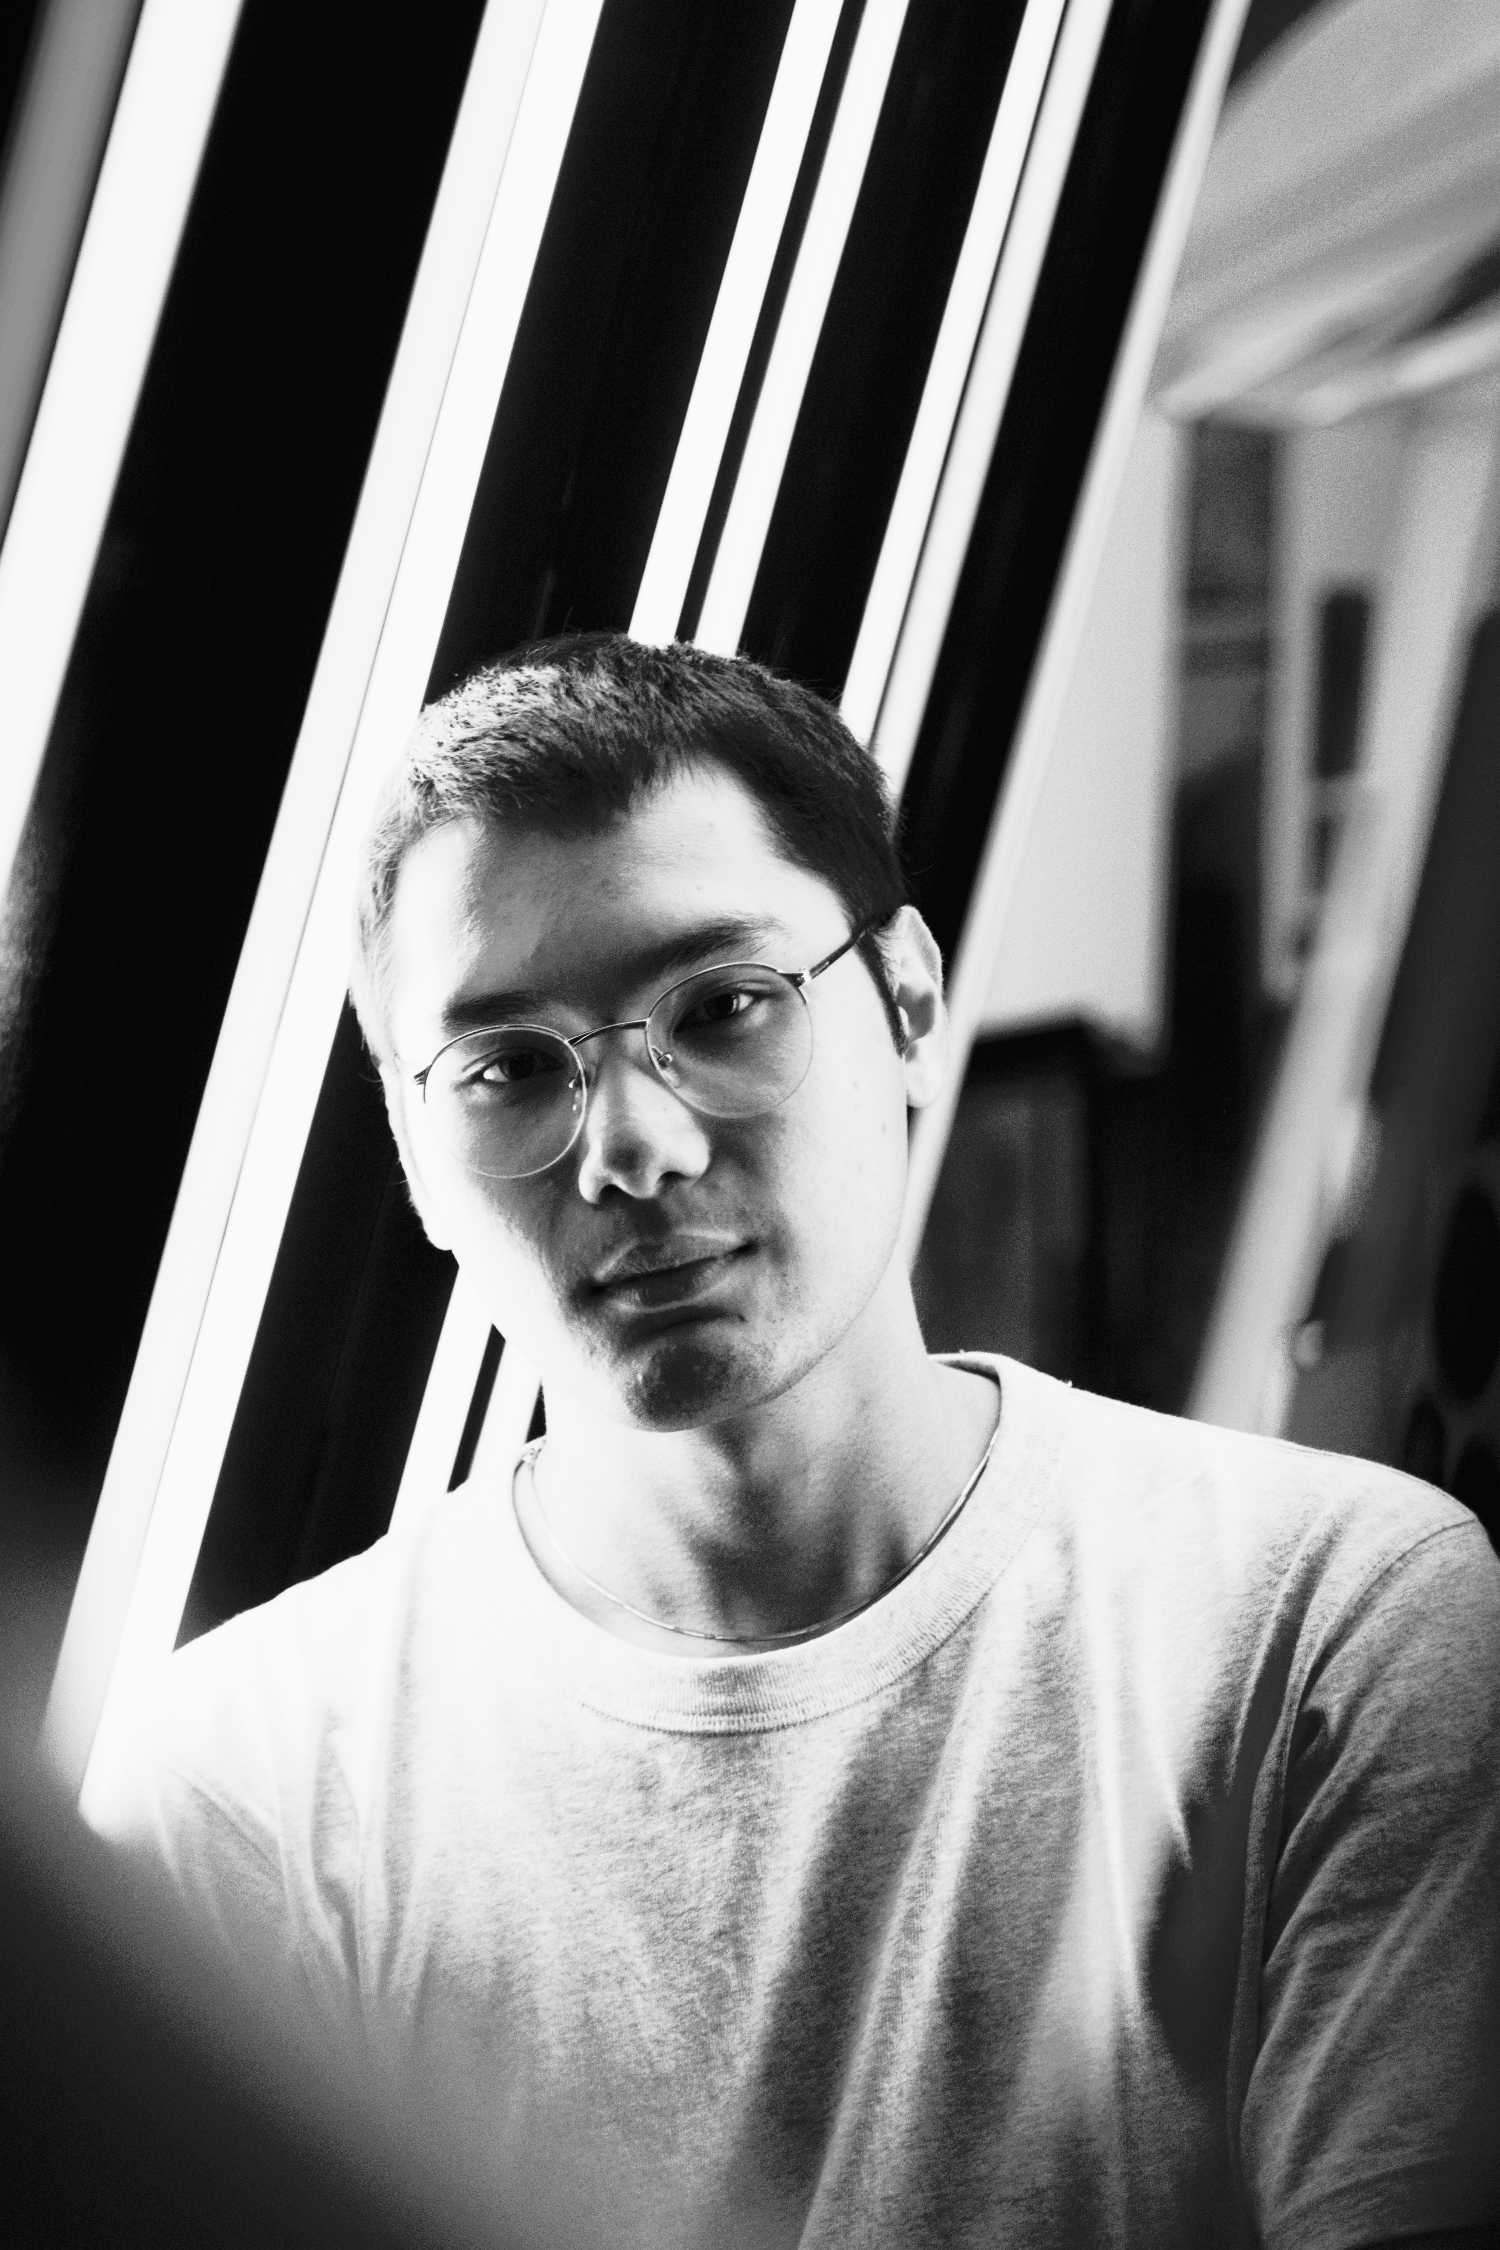
\includegraphics[width=\textwidth]{adapt_eq.png}
		\caption{Nonlinear response}
		\label{fig:adapt-eq}
	\end{subfigure}
	
	\begin{subfigure}[h!]{0.24\textwidth}
		\centering
		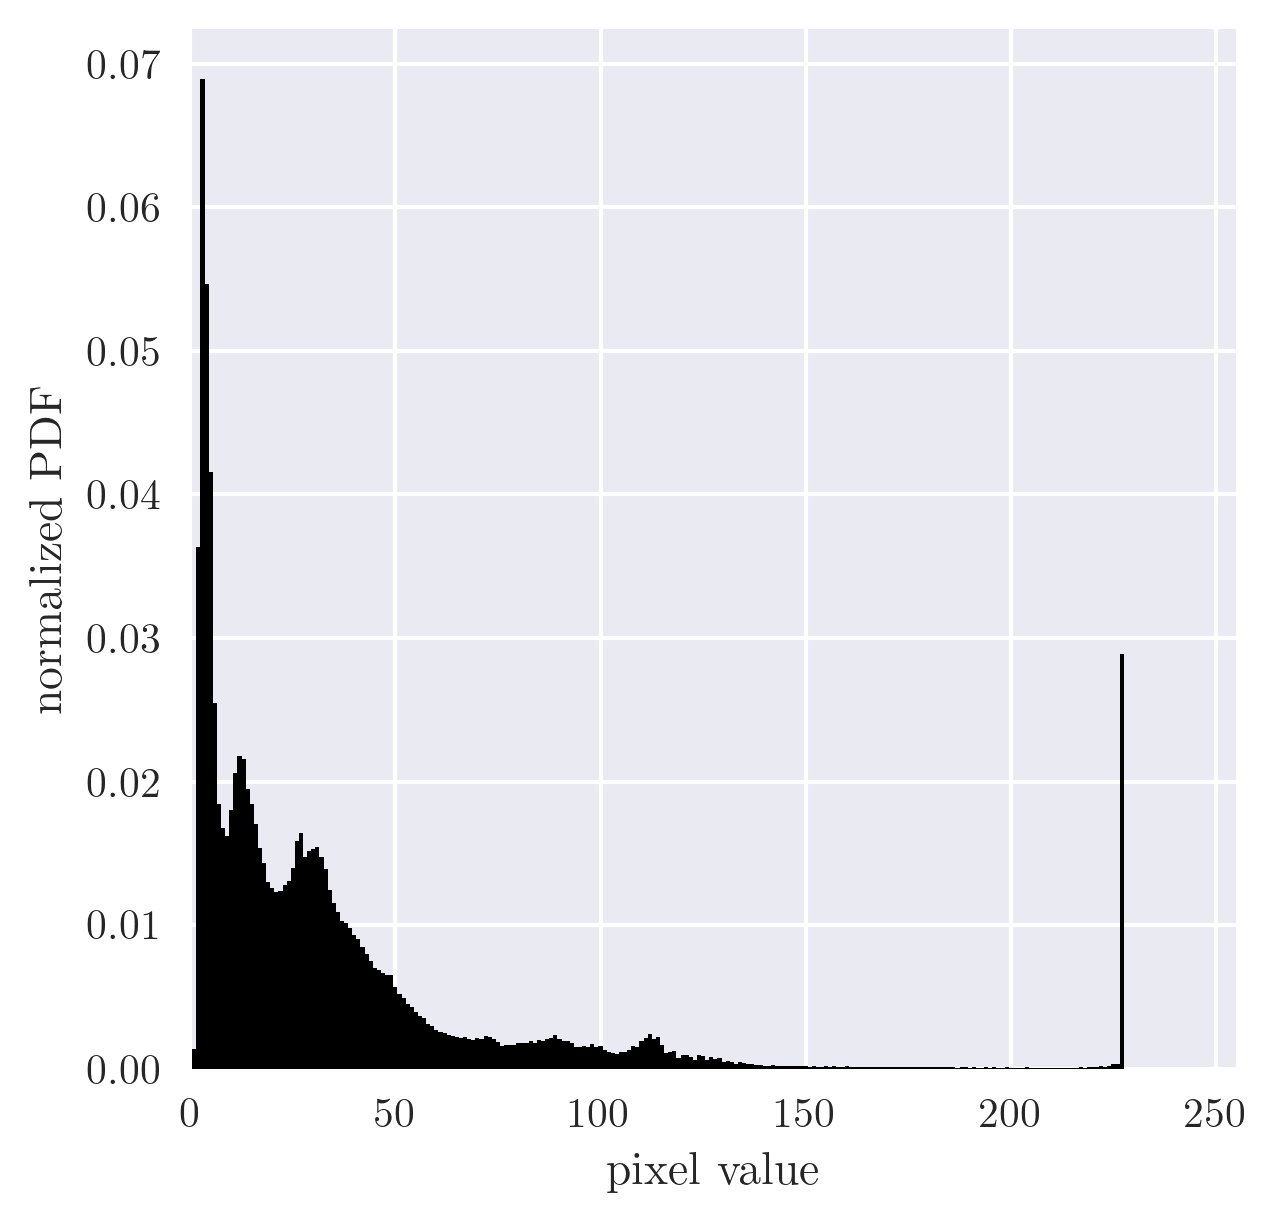
\includegraphics[width=\textwidth]{orig_hist.png}
		\caption{}
		\label{fig:orig-hist}
	\end{subfigure}
	\begin{subfigure}[h!]{0.24\textwidth}
		\centering
		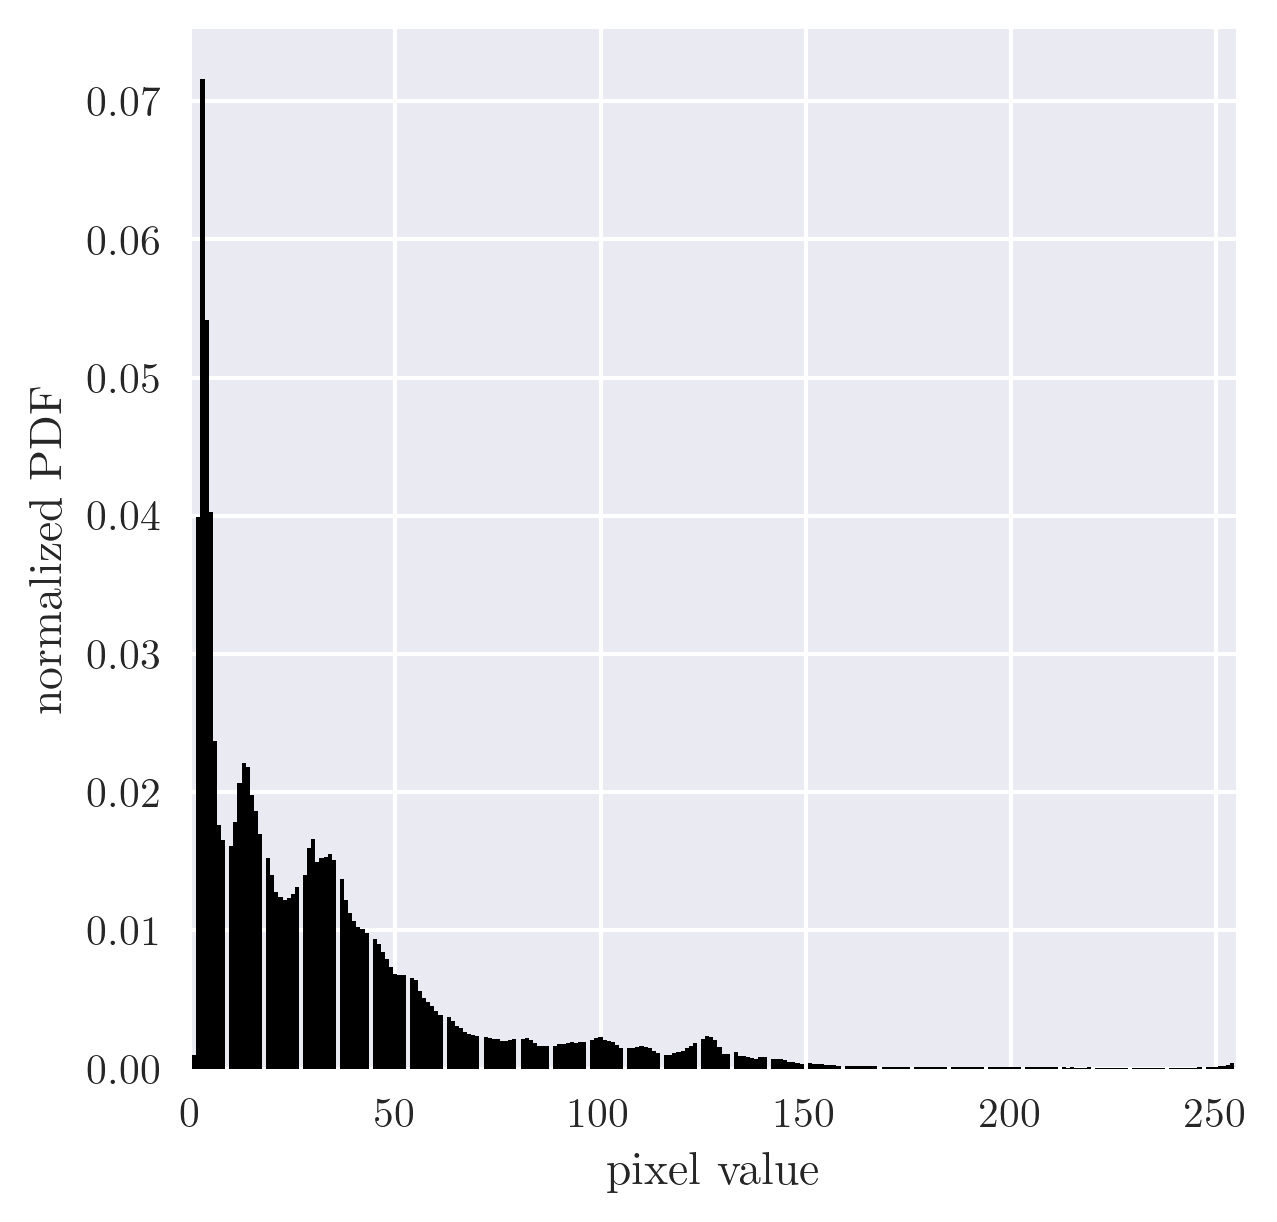
\includegraphics[width=\textwidth]{cs_hist.png}
		\caption{}
		\label{fig:cs-hist}
	\end{subfigure}
	\begin{subfigure}[h!]{0.24\textwidth}
		\centering
		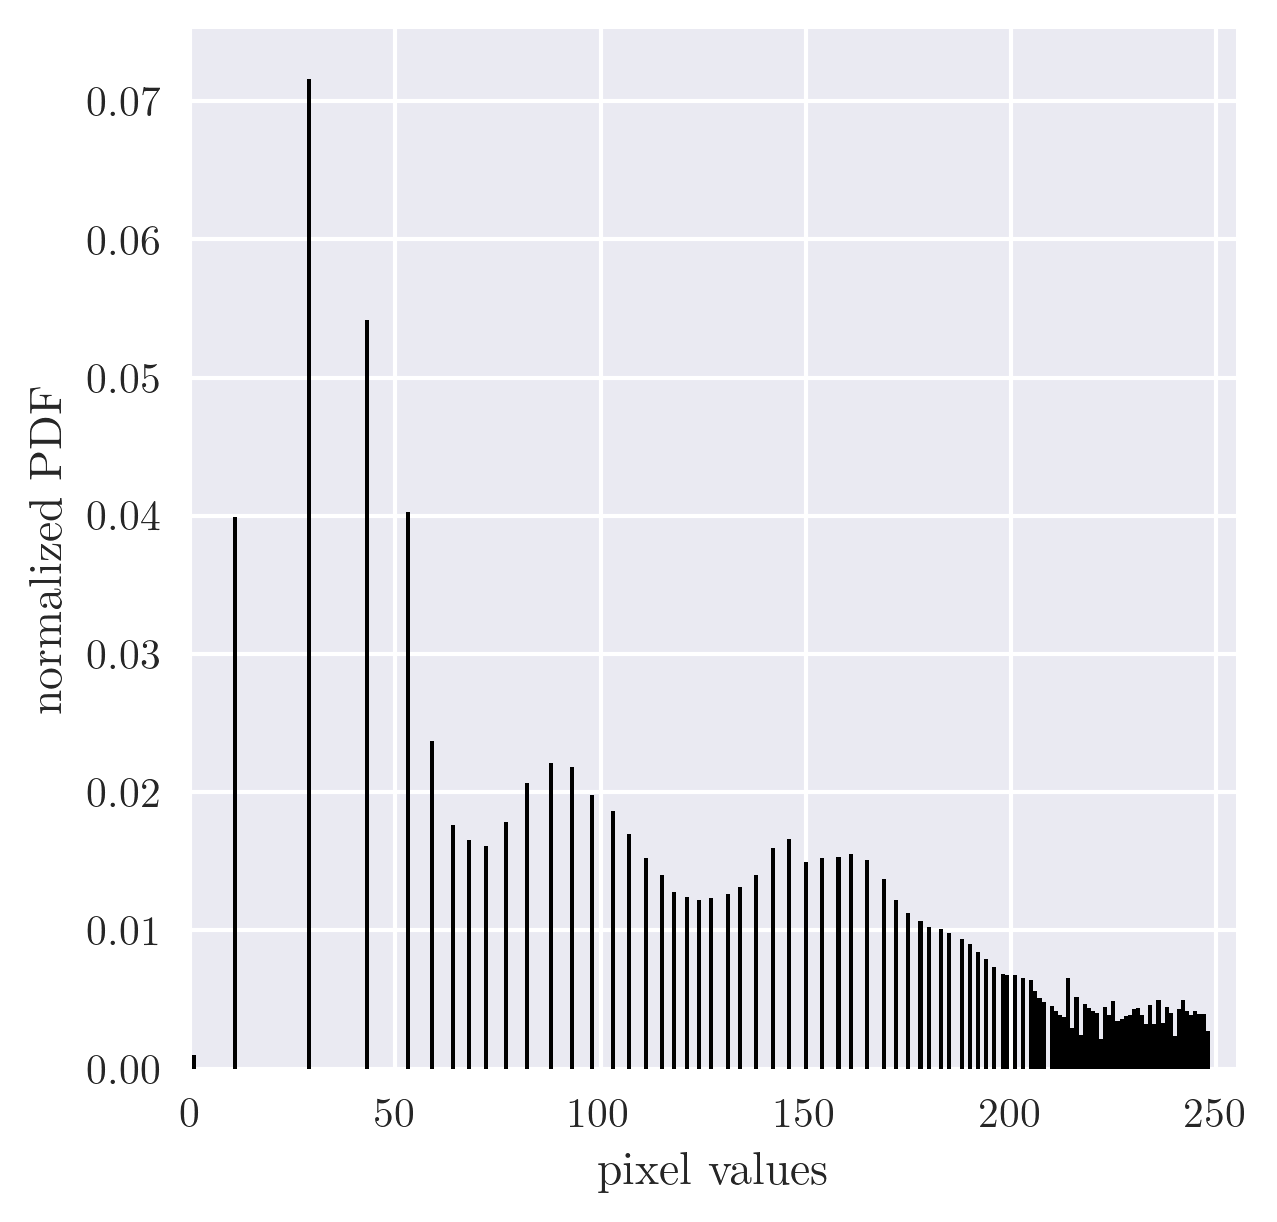
\includegraphics[width=\textwidth]{histeq_hist.png}
		\caption{}
		\label{fig:histeq-hist}
	\end{subfigure}
	\begin{subfigure}[h!]{0.24\textwidth}
		\centering
		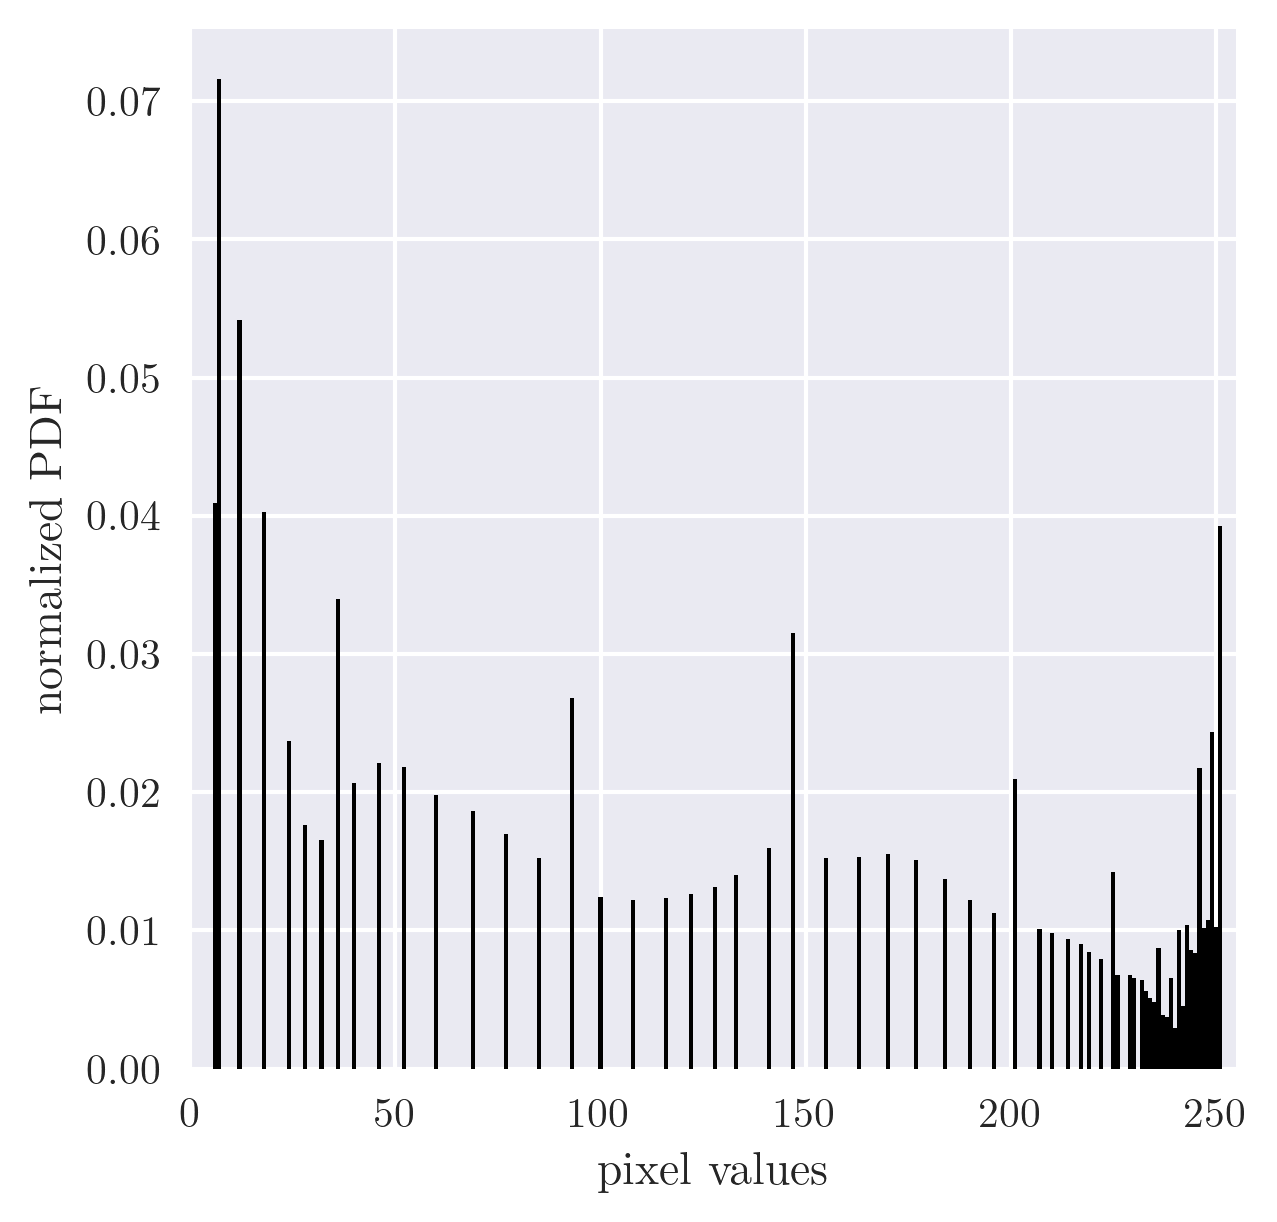
\includegraphics[width=\textwidth]{adapteq_hist.png}
		\caption{}
		\label{fig:adapteq-hist}
	\end{subfigure}
	
	\begin{subfigure}[h!]{0.24\textwidth}
		\centering
		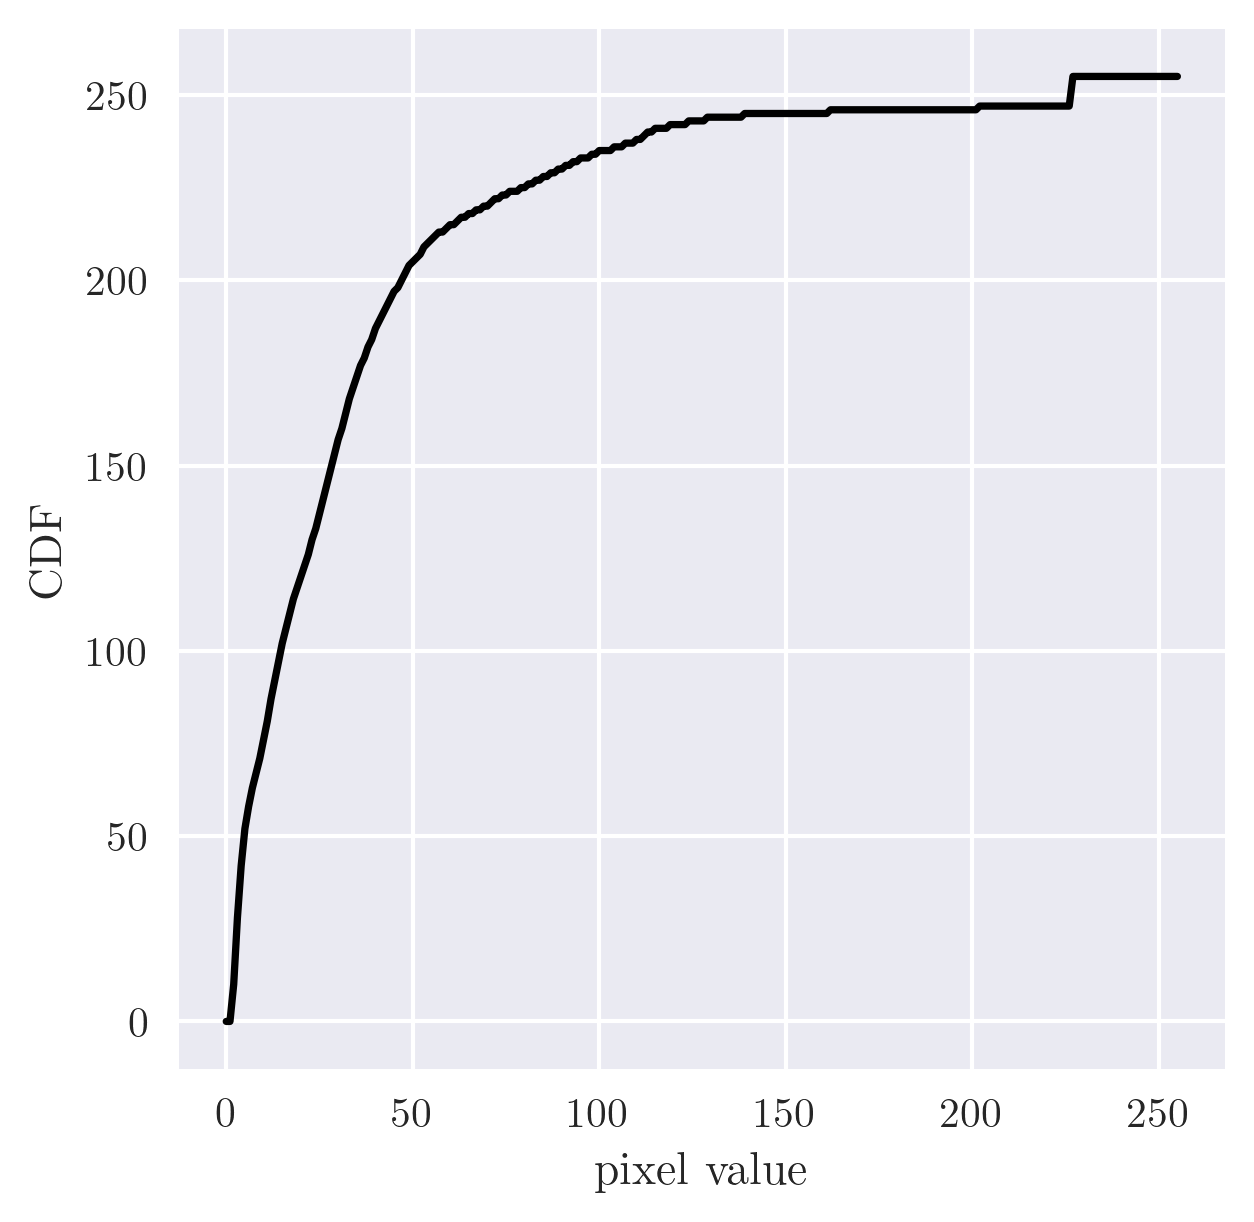
\includegraphics[width=\textwidth]{orig_cdf.png}
		\caption{}
		\label{fig:orig-cdf}
	\end{subfigure}
	\begin{subfigure}[h!]{0.24\textwidth}
		\centering
		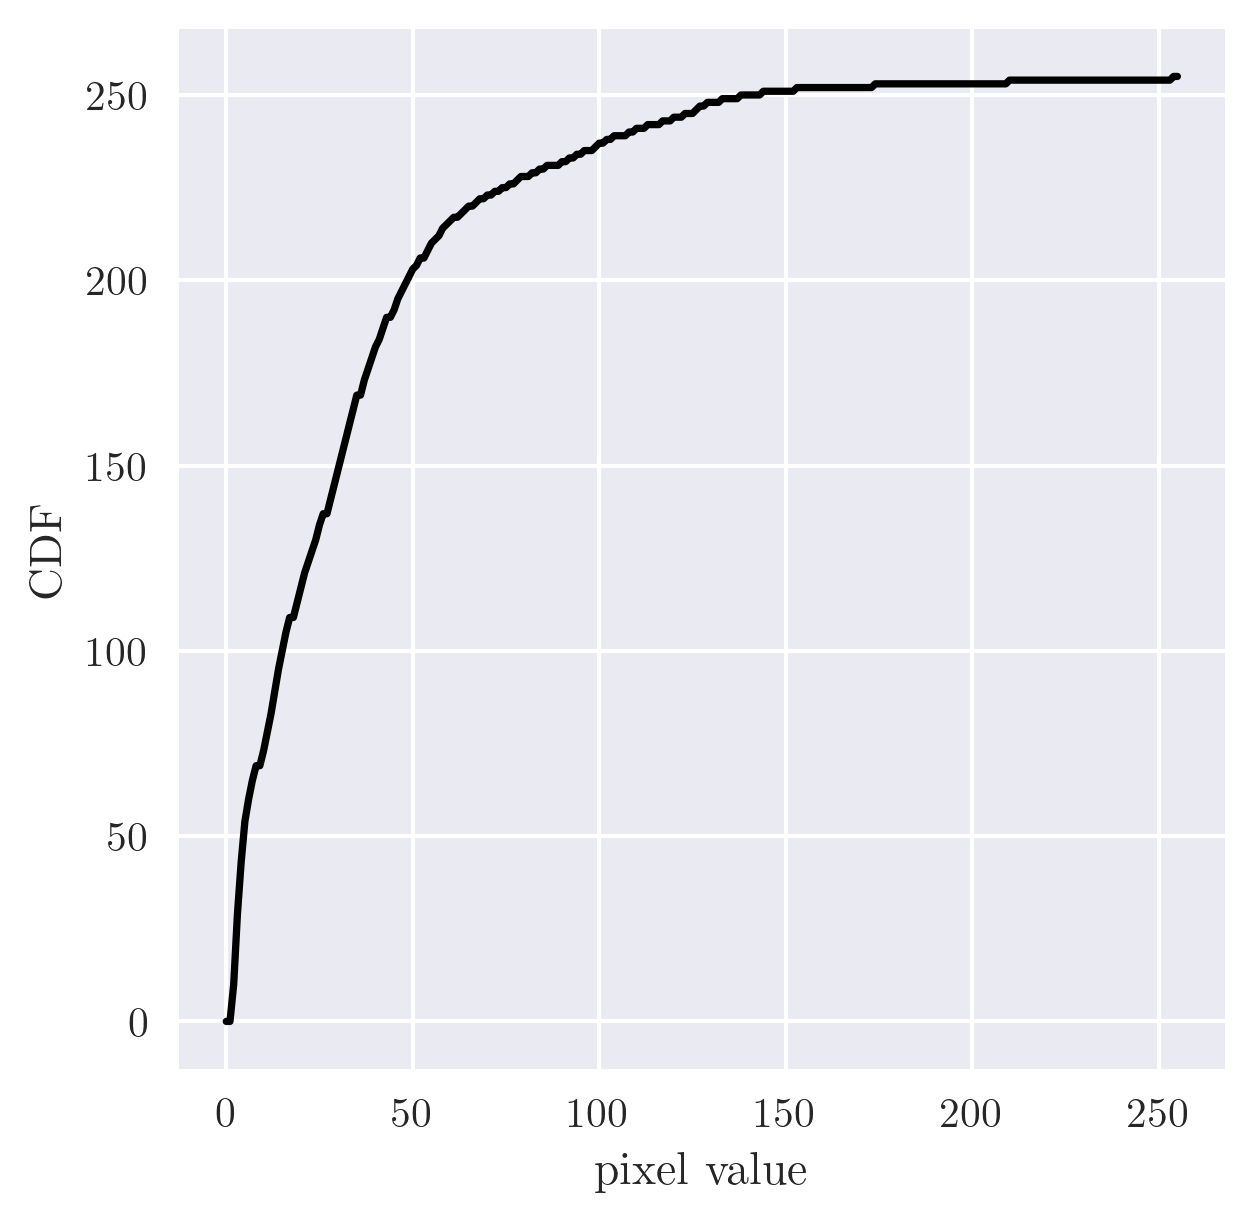
\includegraphics[width=\textwidth]{cs_cdf.png}
		\caption{}
		\label{fig:cs-cdf}
	\end{subfigure}
	\begin{subfigure}[h!]{0.24\textwidth}
		\centering
		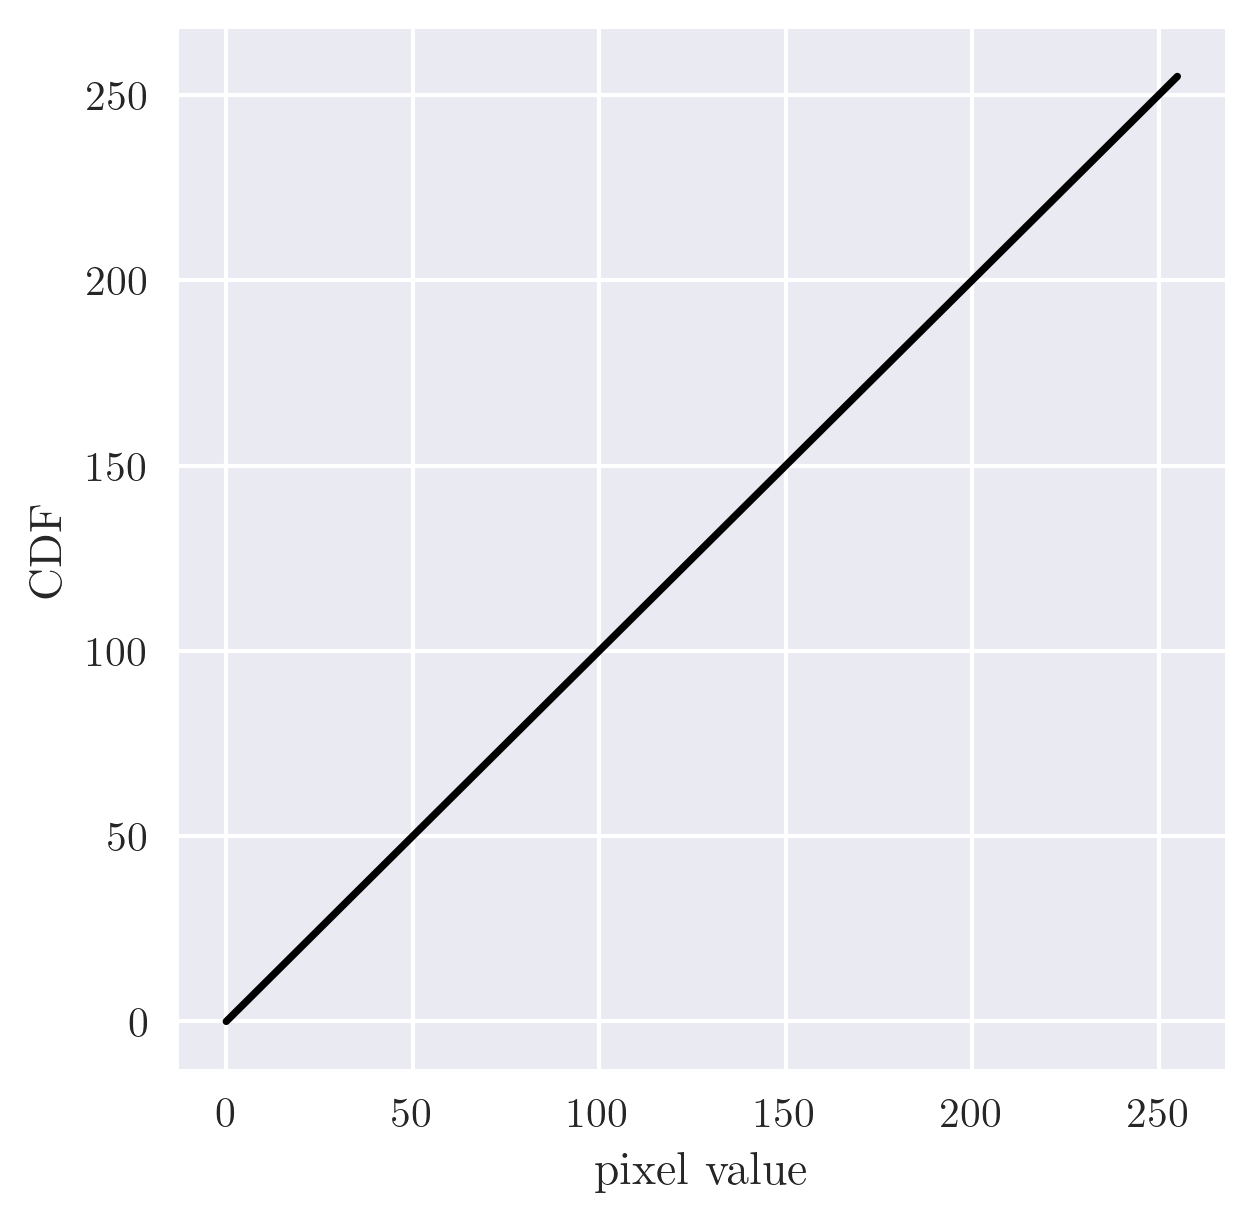
\includegraphics[width=\textwidth]{uniform_cdf.png}
		\caption{}
		\label{fig:histeq-cdf}
	\end{subfigure}
	\begin{subfigure}[h!]{0.24\textwidth}
		\centering
		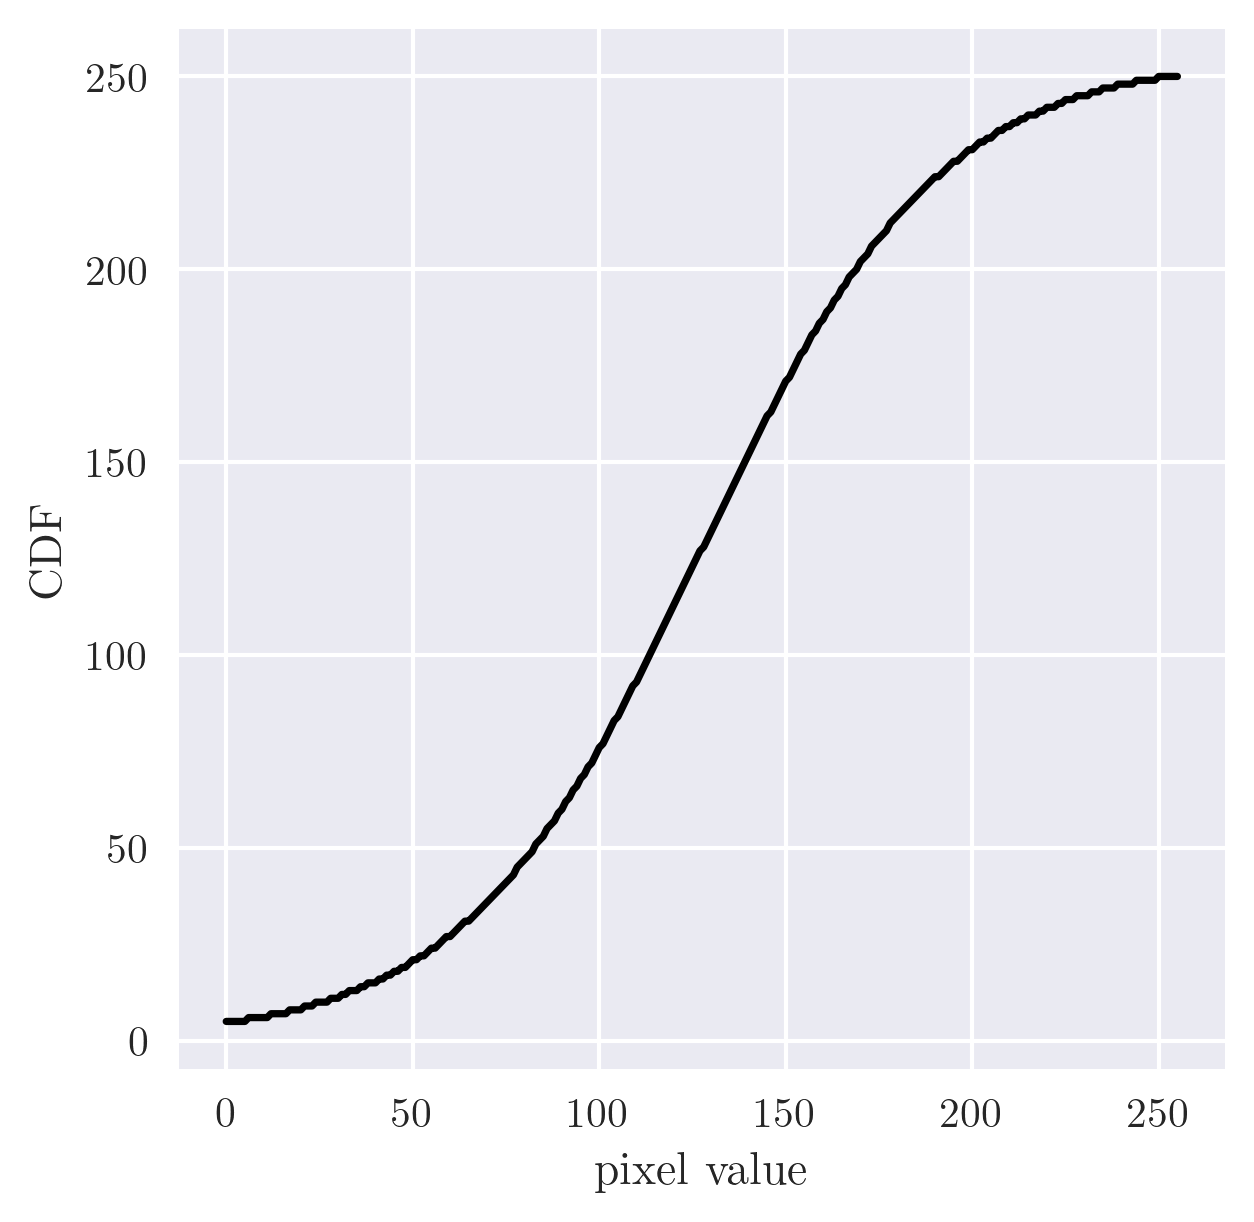
\includegraphics[width=\textwidth]{sigmoid_cdf.png}
		\caption{}
		\label{fig:adapteq-cdf}
	\end{subfigure}
	\caption{Grayscale-converted image and its histogram manipulations (top), their respective histograms (middle), and their respective CDFs (bottom).}
	\label{fig:images}
\end{figure}

\begin{figure}
	\centering
	\begin{subfigure}[h!]{0.33\textwidth}
		\centering
		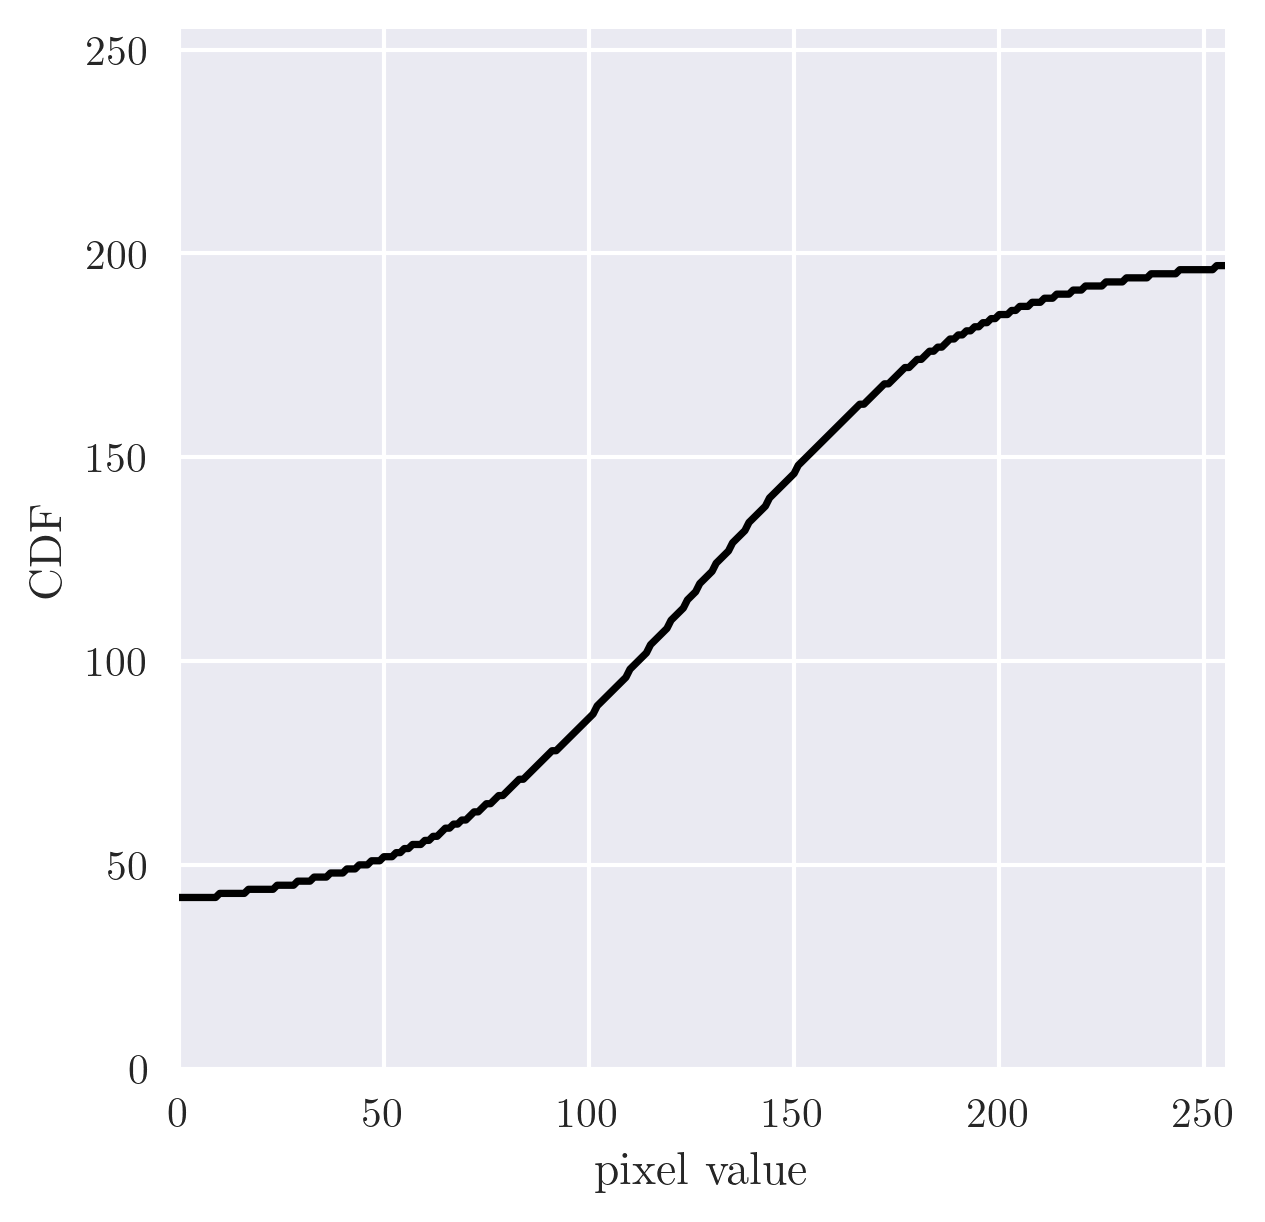
\includegraphics[width=\textwidth]{crush_cdf.png}
		\caption{Desired CDF}
		\label{fig:crush-cdf}
	\end{subfigure}
	\begin{subfigure}[h!]{0.24\textwidth}
		\centering
		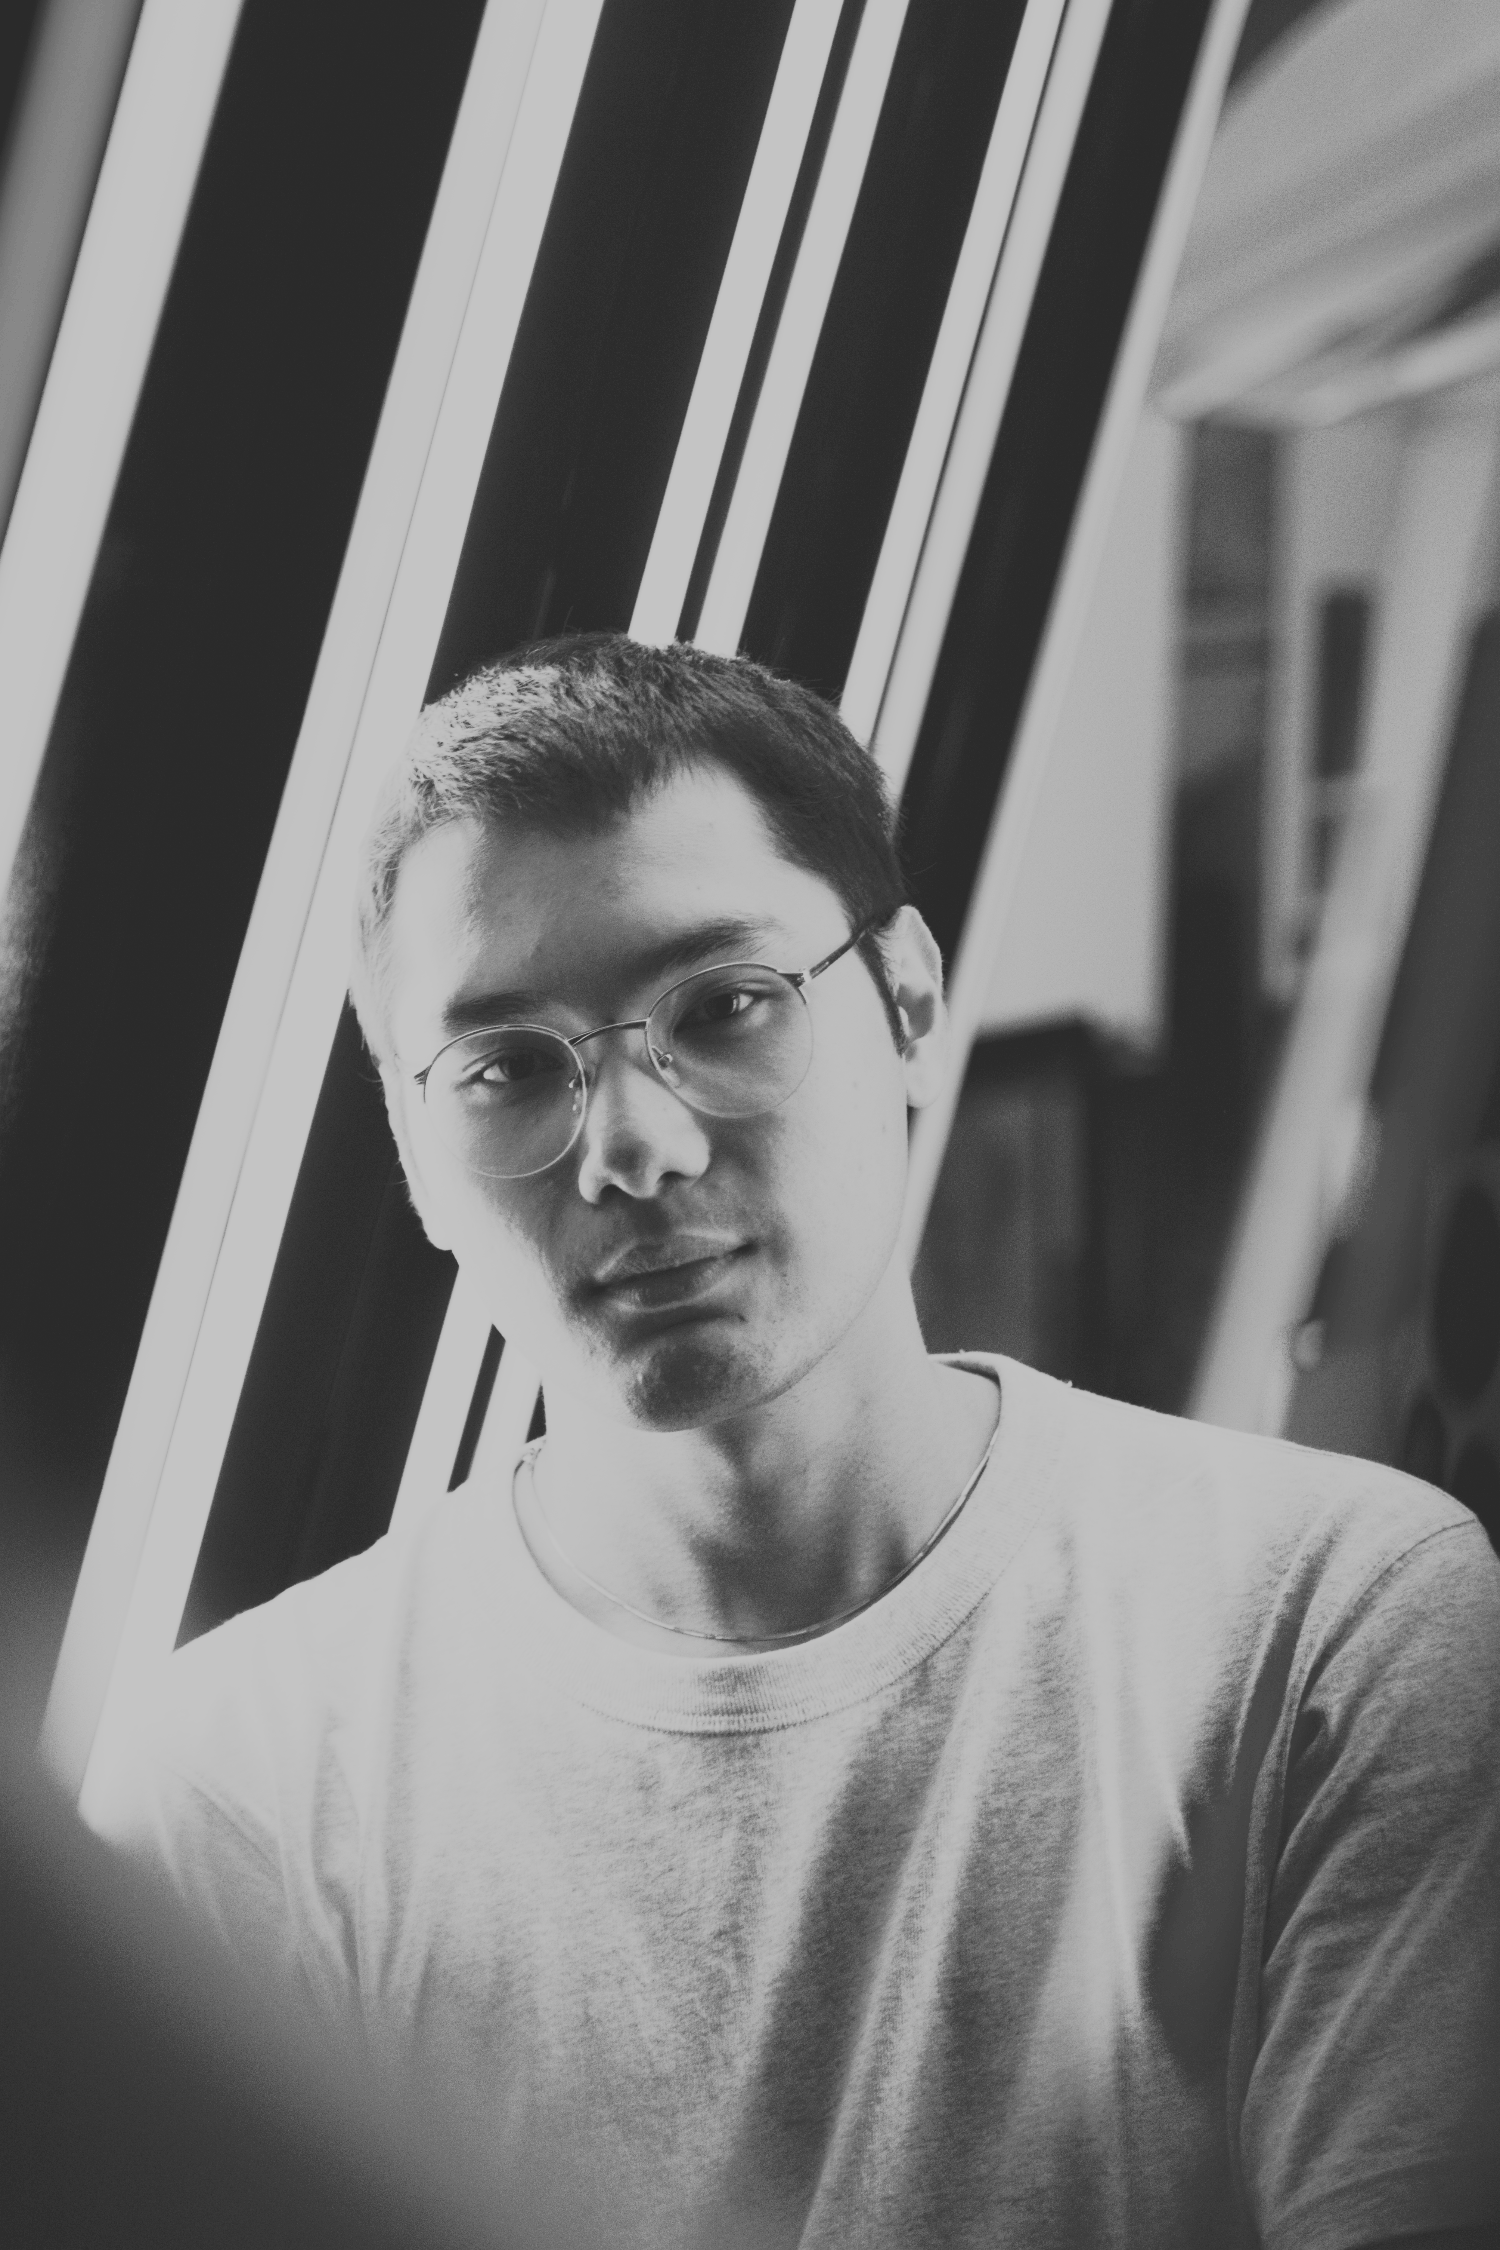
\includegraphics[width=\textwidth]{crushed.png}
		\caption{Resultant image}
		\label{fig:crushed}
	\end{subfigure}
	\begin{subfigure}[h!]{0.33\textwidth}
		\centering
		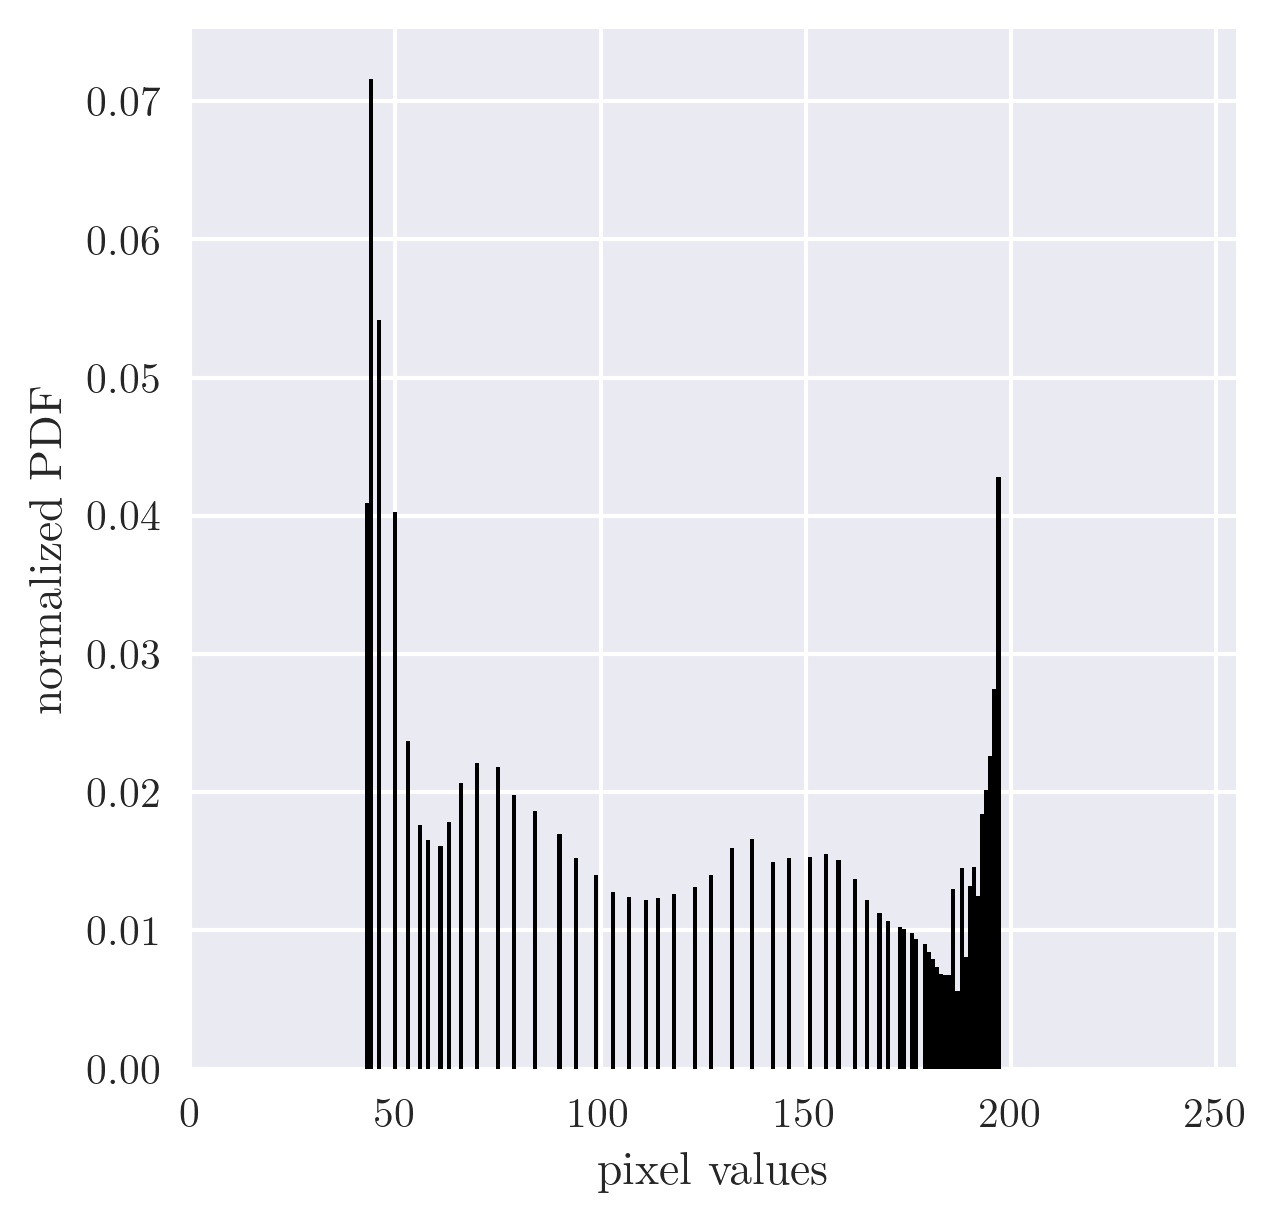
\includegraphics[width=\textwidth]{crush_hist.png}
		\caption{Histogram}
		\label{fig:crush-hist}
	\end{subfigure}
	\caption{``Crushed blacks/whites'' post-processing technique using histogram manipulation.}
	\label{fig:crushed-blacks}
\end{figure}

\begin{table}[!htb]
	\centering
	\caption{Self-evaluation.}
	\begin{tabular}{|r|c|}
		\hline
		Technical correctness & 5 \\ \hline
		Quality of presentation & 5 \\ \hline
		Initiative & 2 \\ \hline
		\textbf{TOTAL} & \textbf{12} \\ \hline
	\end{tabular}
	\label{tab:self-eval}
\end{table}

\bibliographystyle{spp-bst}
\bibliography{186-Act5}

\end{document}